\subsection{Brugerovervejelser}
\label{brugerovervejelser}
Da dette projekt handler om at udvikle et system til at hjælpe skolerne med deres skemalægning, nytter det ikke noget at lave et system de ikke kan gennemskue, og dermed bruge. Derfor er det relevant at kigge på brugernes færdigheder i forhold til at benytte informationssystemer.

På figur \ref{fig:docendo_skema} er skemalægningsprogrammet Docendo vist. Dette program blev tidligere brugt på Kærbyskolen og som det kan ses på figuren bruges der drag\&drop til at indsætte moduler i skemaet. Dette gør programmet meget intuitivt og let at bruge, noget som Kærbyskolen efterspørger. I interviewet med Kærbyskolen fortalte skemalæggeren at programmet skulle være meget let at bruge, for at det var en god løsning for skolen.

\begin{figure}[h!]
	\centering
	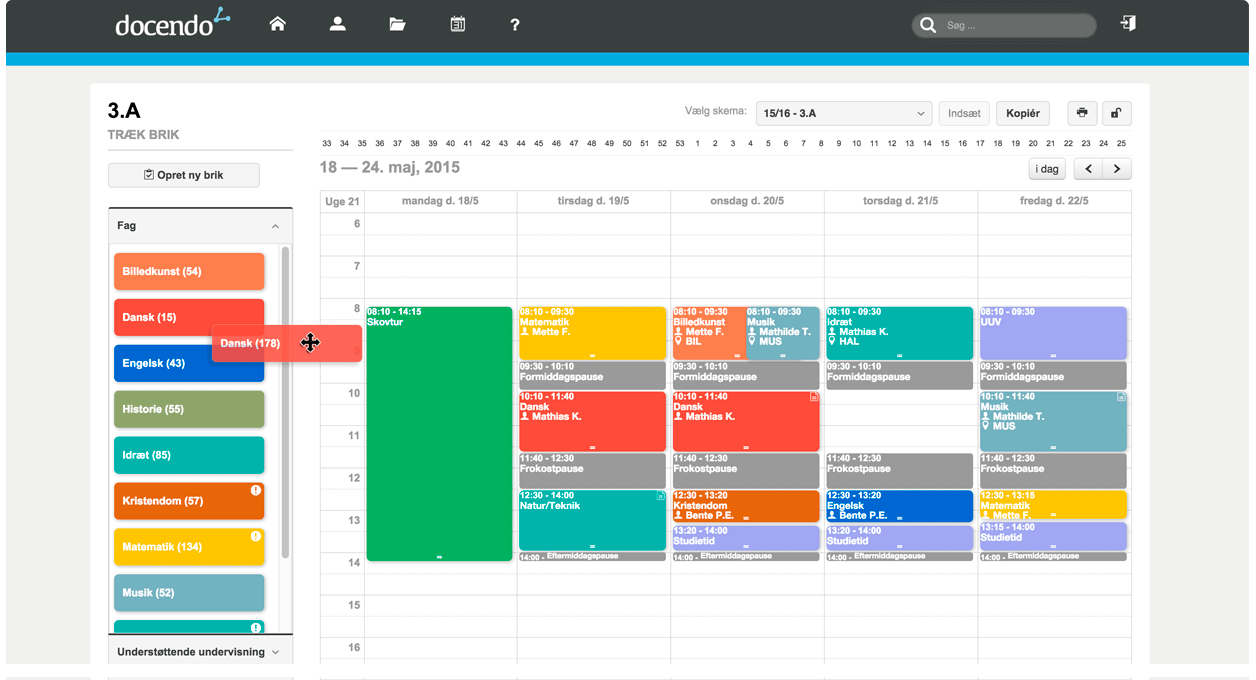
\includegraphics[width=\textwidth]{Docendo}
	\captionsource{Docendos skemalægningsprogram}{\url{https://docendo.dk/folkeskole.html}}
	\label{fig:docendo_skema}
\end{figure}

På skolen er der flere forskellige systemer der skal arbejde sammen for at fungere. Skemaet skal eksempelvis lægges ind på nettet i SkoleIntra, så eleverne kan få adgang til det. Derfor er det vigtigt at et eventuelt program der laves til at hjælpe med denne skemalægning, er kompatibelt med disse allerede eksisterende programmer, så der ikke skal manuelt arbejde til at konvertere filer fra det ene system til det andet. Heldigvis bruges der i de fleste programmer CSV-filer, hvilket er tekstfiler med kommasepareret værdier, som så kan læses af de respektive programmer. Det der gør denne filtype nem at arbejde med, er at ved at udskrive informationer omkring skemaet i forskellige rækkefølger, men i samme filformat, kan vi eksportere til alle disse programmer.

Ved at lave en måde at eksportere på til de forskellige formater, kan skemaet tages direkte fra vores program, og sættes ind i de andre programmer. Dette betyder for skolen at programmet potentielt kun skal bruge informationer omkring skolen og lærere, og så kan den selv lave et skema der er klar til at de kan bruge det direkte.

Interviewet med Tingstrup skole fortalte, at det ikke var nødvendigt med en grafisk brugerflade, så længe at der var noget som fortalte brugeren hvad programmet lavede. Det vil sige at det ikke er nødvendigt at have flot grafik, så længe brugeren kan se programmets status. 

Det vil sige, at kravet fra de to skoler er et system som ikke behøves at have en grafisk brugerflade, men som skal være nemt at bruge, samtidig med at det hele tiden skal oplyse om hvor langt det er, så brugeren (skemalæggeren) kan se om systemet er gået i stå, eller om der er opstået problemer. Når programmet skal laves, er det altså vigtigt det holdes for øje at brugerne af systemet ikke nødvendigvis ved hvad de skal, og at programmet derfor skal guide dem igennem processen med at indtaste data.